\mav{Briefly introduce Gibbon again}

\mav{Make clear that the Gibbon compiler is a collaborative project, of which I was one
  member, though my contributions to it are major (wording?) so in this section I'll use
  a lot of ``we''}

\section{Converting Functional Programs to the Location Calculus}\label{sec:infer-local}

\ourcalc captures a notion of computation over (mostly) serialized data,
\emph{exposing} choices about representation. It provides the levers needed by a human
or another tool to explore the design space of optimization trade-offs above
this level, \ie{} for the human or tool to answer the question
\emph{``how do we globally optimize a pipeline of functions on serialized data?''}.

%\begin{itemize}
%\paragraph{How to globally optimize pipelines of functions on serialized data?}
%  \begin{itemize}
   First, if multiple functions use the same datatype, do they standardize on one
    representation?  Or does that datatype take different encodings at different
    points in the pipeline (implemented by cloning the datatype and
    presenting it to \ourcalc with different annotations)?
%
    Second, when up against the constraint of {\em already-serialized} data on
    disk, the compiler can't change the existing representation, if the
    external data \emph{lacks offsets}, is it better to \emph{force}
    the first consuming function to use that representation, or to insert an
    extra {\em reserialization} step to convert\footnote{Still faster
    than traditional deserialization: no object graph allocation.}?
%
    Third, can the compiler permute fields to improve performance or reduce the
    stored offsets needed?
%  \end{itemize}
%\end{itemize}

% This large space of future work is beyond the scope of this paper, but we nevertheless
% illustrate the process of
% integrating \ourcalc into Gibbon.

    All of these choices can be represented directly in \ourcalc, making it an
    ideal intermediate language for a compiler. This chapter will describe Gibbon,
    an experimental compiler that transforms functional programs to work on
    (mostly) serialized data. Gibbon represents its programs in \ourcalc,
    performing various analyses and transformations, then generates low-level C code.
%% building a front-end above \ourcalc with one example
%% tool: the {\em \lamadt} language and compiler.
%
The front-end language for Gibbon, \lamadt, is a vanilla purely functional
language without any region or location
annotations.  It hides data-layout from the programmer (and the low-level
control that comes with it).  It also facilitates comparison with
mature compilers, as \lamadt runs standard functional programs:
for example, the {\em unannotated} examples we've seen in this paper.

{The syntax for \lamadt is a subset of Haskell syntax, supporting
  algebraic data types and top-level function definitions. It is a
  monomorphic, strict functional programming language, and for
  simplicity it is first order, like \ourcalc.}
% \mv{Future work: closures?}
{In future-work, the plan is to add support for a higher-order, polymorphic
  front-end language through standard monomorphization and defunctionalization.
  (An interesting consequence of this will be that closures become regular
  datatypes, such that a list of closures could be serialized in a dense
  representation.)}

%% \mav{Using multiple representations for the same type in the same program is an area
%% for future study.
%% \Secref{sec:eval} includes the multi-pass program \il{repmax}
%% where one pass incurs overhead to satisfy the representation needs of another.
%

\paragraph{Implementing \lamadt}
The compiler must perform a variant of {\em region
  inference}~\cite{regioncalcs,mlkit-retrospective}, but differs from
previous approaches in some key ways.
%
The inference procedure uses a combination of standard techniques from the literature and specialized
approach for satisfying \ourcalc's particular needs\footnote{The {\em
    Directed Inference Engine for region Types}, if you will.}.
%
Because the inference must determine not only what region a value belongs to,
but \emph{where} in that region it will be, the inference procedure returns a
set of constraints for an expression similar to the constraint environment used
in the typing rules in \figref{fig:types1} and \figref{fig:types2}, which are
used to determine placement of symbolic location bindings. Additionally, certain
locations are marked as \emph{fixed} (function parameters, data constructor
arguments), and when two fixed locations attempt to unify it signals the need
for an indirection, and the program must be transformed accordingly.

Our current implementation adds an extra variant to every data type
\footnote{These indirections do double-duty in allowing the memory
  manager to use non-contiguous memory slabs for a region \secref{subsec:rts}.}
representing a single indirection (called \il{I}).  For example, a binary tree
\il{T} becomes
\begin{code}
data T = Leaf | Node T T | I (Ind T)
\end{code}
%
The identity function \il{id x = x}, when compiled to \ourcalc, is \il{id x = I x}.
Likewise, sharing demands indirections, and
\il{let x = _ in Node x x}
becomes
\il{let x = _ in Node x (I x)}.
%
%% For it to {synthesize} a well-typed \ourcalc term, it adds
%% indirections (not offsets) to satisfy two constraints: (1) a function
%% must write its output to distinct destination region(s) passed as arguments,
%% and (2) a data-constructor must have all its arguments within the same region,
%% consecutively ordered by location.
%
%% For example, these problems arise in compiling the following functions:
%% \begin{code}
%%   id x = x
%% shareTree 0 = Leaf 1
%% shareTree n = let x = shareTree (n-1) in
%%               Node x x
%% \end{code}

%% In the case of the identity function, the fixed locations of the
%% function type prevent the program from returning a value of the same
%% location as its input, so it must be transformed to instead return a
%% location in a new region that consists of an indirection to the
%% input. Similarly, in the second function, because the same subtree is
%% used twice (shared) as both fields of a node, the node constructor
%% will be annotated to expect indirections for both fields.
%For example, the identity function becomes:


\section{Compiling the Location Calculus} \label{sec:impl-local}

In this section we present a compiler for the \ourcalc language, which consists of
the formalized core from~\secref{subsec:grammar}, extended with various primitive types, tuples,
convenience features, and a standard library.
%
A well-typed \ourcalc program guarantees correct handling of regions, but the
implementation still has substantial leeway to further modify datatypes and
the functions that use them.
%
By default, the compiler we present inserts enough indirection in
datatypes to preserve the asymptotic complexity of the source functions (under
the assumption of $O(1)$ field access), but we also provide a mode---activated
globally or per-datatype---that leaves the data types
\emph{fixed} and instead introduces inefficient ``dummy traversals'' and copying
code into compiled functions.
%
%% (In this mode, our compiler produces a similar result to what Gibbon produced
%% previously~\cite{ecoop17-gibbon}---for comparison, we will distinguish between
%% Gibbon2 (with \ourcalc) and Gibbon1 (without \ourcalc) in~\secref{sec:eval}.)
%
%% Where the formal presentation of the language relied on the end witness judgment
%% to reach the end of sub-trees, a proper compiler need to actually generate
%% efficient code that avoids unnecessary traversals. To do this, we make use of
%% some of the compilation strategies described in~\cite{ecoop17-gibbon}, namely
%% making explicit the threading of end-witnesses through recursive programs and
%% the subsequent lowering of programs to a ``cursor-passing'' form.

{Note that this ``inflexible'' mode---which doesn't allow the compiler to
  insert indirections---is also used when reading in external data.  In our
  \ourcalc implementation, we provide a mechanism for any datatype to be read
  from a file (via \il{mmap}),whose contents are the pointer-free, full
  serialization.  We use the same basic encoding as Haskell's
  \il{Data.Serialize} module derives by default, but plan to extend it in the
  future.}

Ultimately, because \ourcalc is meant to be generated by tools as well as programmers,
its goal is to add value in both safety and performance, but to leave
\emph{open} the design space of broader optimization questions to a front-end that
targets \ourcalc{}. One example of such a front-end tool is the front-end of
Gibbon, as described previously in \secref{sec:infer-local}.

%\floatstyle{boxed}\restylefloat{figure}
\begin{figure}
  %% \small
  \begin{displaymath}
    \begin{aligned}
      &n \in \; \textup{Integers}
    \end{aligned}
  \end{displaymath}
  \begin{displaymath}
    \begin{aligned}
      \textup{Types} && \TYP && \gramdef & \ldots \gramor \gramwd{Cursor} \gramor \gramwd{Int} \\
      \textup{Pattern} && \spat && \gramdef & \caseclause{\datacon{\DC}{}{(\var : \gramwd{Cursor})}}{\EXPR} \\
      \textup{Expressions} && \EXPR && \gramdef & \dots \\
      && && \gramor & \switch{\var}{\spat}\\
      && && \gramor & \readInt{\var} \gramor \writeInt{\var}{n} \\
      && && \gramor & \readTag{\var} \gramor \writeTag{\var}{\DC} \\
      && && \gramor & \readCursor{\var} \\
      && && \gramor & \writeCursor{\var}{\concreteloc{r}{i}{l}} \\
    \end{aligned}
  \end{displaymath}
  \normalsize
  \caption{{Grammar of \lamcur{} (an extension of \ourcalc{}) \captionscrunch}}
  \label{fig:nocal-grammar}
\end{figure}

\subsection{Compiler Structure}\label{subsec:compiler_structure}
We implement \ourcalc with a micropass, whole-program compiler that performs
full region/location type checking
%% (and running test programs)
between every pair of passes on the \ourcalc intermediate representation (IR).
%
% The most important intermediate representations (IRs) are these three:
%\rn{Standardize on whether or not we'll use the term Cursor.}
% => WE ARE!
%
After a series of \ourcalc$\rightarrow$\ourcalc passes, we lower to a second IR,
\emph{\lamcur}.
As shown in \figref{fig:nocal-grammar},
\lamcur is not a calculus at all, but a low-level language where
memory operations are made explicit.  \lamcur{} functions closely resemble the C++
code shown early in Chapter~\ref{chapter:intro}.
%
Code in this form manipulates pointers into regions we call {\em cursors} because of
their (largely continuous) motion through regions.
%
{We represent \lamcur internally as a
  distinct AST type, with high level (non-cursor) operations excluded.}

Within this prototype compiler, tuples, and built-in scalar types like Int, Bool
etc. are \emph{unboxed} (never require indirections).
%
In the following subsections, we describe the
% \ourcalc ($\rightarrow$ \ourcalc)* $\rightarrow$ \lamcur{}
compiler in four stages.
{Similar to \lamcur, our compiler represents
  programs at these stages with AST types that track changes in the
  grammar needed by each pass.
  After these four steps,}
  the final backend is completely standard.  It eliminates
tuples in the \emph{unariser},
% (for more easily generating efficient C code)
performs simple optimizations, and generates C code.
%
Because of inter-region indirections, a small \ourcalc runtime system is
necessary to support the generated code.

The \ourcalc runtime system is responsible for region-based memory management.
A detailed description of the memory management strategy is available in \secref{subsec:rts} %Appendix~\appendixref{chapter:rts}.
In brief, we use region-level reference counts.  Each region is implemented as
linked list of contiguous memory chunks, doubling in size.  This memory is write-once,
and immutability allows us to track reference counts \emph{only} at the region
level.  Exiting a \il{letregion} decrements the region's count, and it is freed
when no other regions point into it.

\begin{figure*}\center
  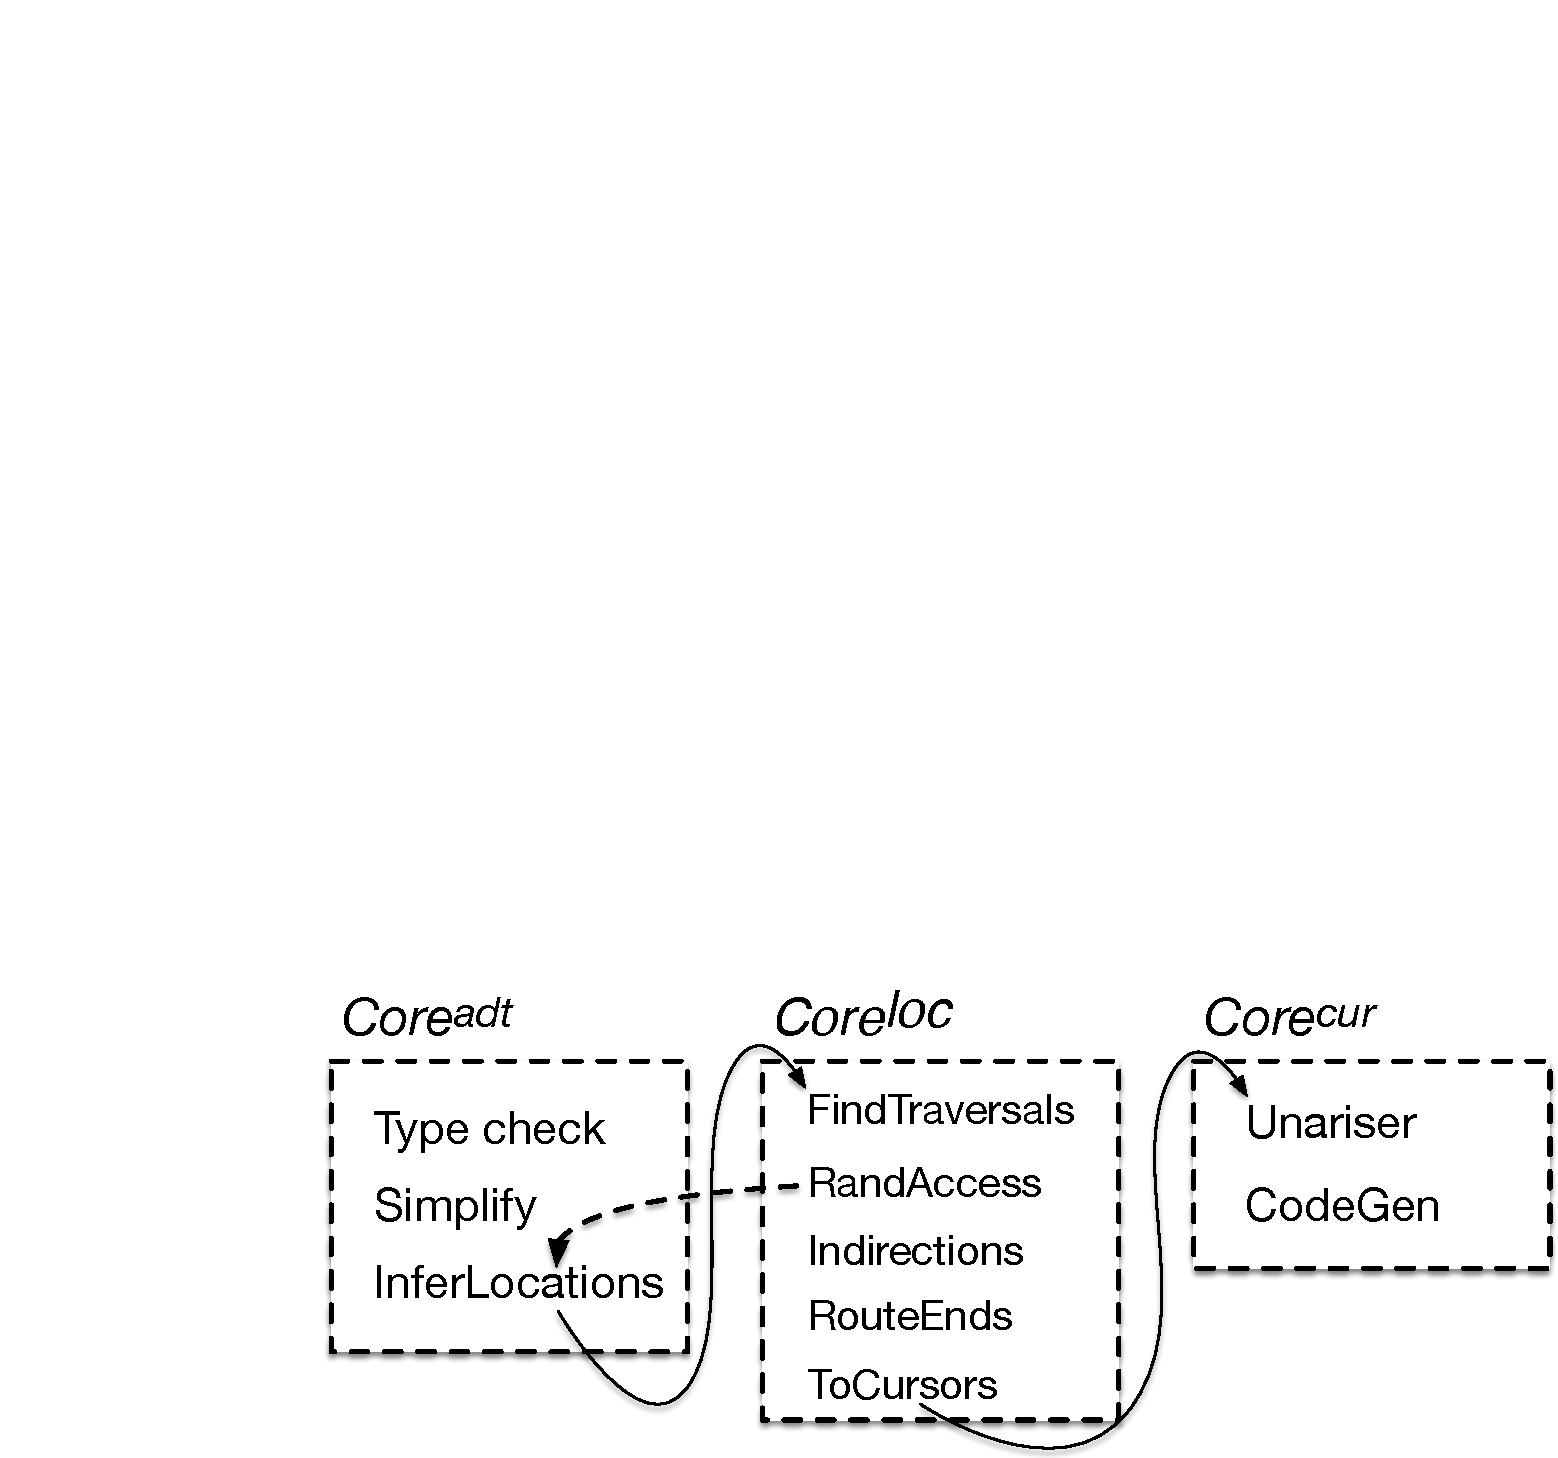
\includegraphics[width=0.6\textwidth]{compiler_arch}
  \caption{Compiler architecture.  Here we show the most important
    passes within the three phases of the compiler delimited by
    the three core IRs (front-end, middle-end, back-end).}
  \label{fig:compiler-arch}
\end{figure*}

\subsubsection{Finding Traversals}
\label{sec:find-traversal}

%% After location inference produces a valid \ourcalc{} program, the program is
%% still in a form that assumes access to any field of a data constructor.

%% In order to efficiently compile expressions with pattern matching on data
%% structures {with one or more fields which are not indirections}, the
%% compiler needs to generate code for computing the pointers of each field of the
%% structure in order to bind them to pattern variables.

Pattern matches in \ourcalc bind all constructor fields, including those that
occur at non-constant offsets, later in memory.
%
The compiler must determine which fields are reachable based on either (1)
constant offsets, (2) stored offsets/indirections present in the datatype, or
(3) by leveraging traversals already present in the code that scan past the
relevant data.
%
The third case corresponds to determining end witnesses in the formal semantics.
%% and in general \ourcalc{} allows for all fields in any
%% data structure to be bound by pattern matching.
%
%% That is, for a pattern match on \il{Node x y}, the program may assume that it
%% can reference \il{y} and therefore (implicitly) compute the end witness of \il{x} to reach
%% the address of \il{y} in memory.
%
% including those to the right of inline-serialized child structures.
Likewise, this compiler pass identifies data reached by the work the program
already performs.

%% %% we have an extremely simple metric for whether it is at risk of increased work
%% %% and degraded asymptotic complexity:
%% %% \begin{itemize}
%% %% \item Was a \il{copy} inserted?
%% %% \item Does the program refer to a location
%% %% \end{itemize}

%% %% After the location inference algorithm generates a \ourcalc{} program,
%% %% we run {a simple analysis to check if the asymptotic complexity of
%% %%   any of the functions has changed},
%% %% \rn{no that's not simple in general!}
%% %% and if it has, we add
%% %% layout information to the program to restore it.
%% %% Since the location inference algorithm applies some `known' program
%% %% repair strategies like inserting calls to copy functions,
%% %% adding dummy traversals etc. performing this analysis is a simple matter
%% %% identifying these repair strategies and
%% %% replacing them with more efficient ones.
%% %% All calls to copy functions can be eliminated just by inserting
%% %% an indirection node instead.
%% %% However, doing the same for traversal functions
%% %% is tricky and requires some further analysis.


To this end, we use a variation of a technique we previously proposed
\cite{ecoop17-gibbon}.  Specifically, we assign \emph{traversal effects} to
functions.  A function is said to {\em traverse} it's input location if it
touches every part of it.  In \ourcalc{}, a case expression is the only way to
induce a traversal effect.  If all clauses of the case expression in turn
traverse the packed elements of the corresponding data constructors, the
expression traverses to the end of the scrutinee.
%
Traversing a location means witnessing the size of the value encoded at that
location, and thus computing the address of the \emph{next} value in memory.
% (This is the $\phi$ function from \secref{sec:lang}).
%
After this pass, the type schemes of top-level function definitions reflect
their traversal effects.

%% This analysis is very similar to the \emph{effect inference} process
%% described in~\citet{ecoop17-gibbon}.
%% % , and we leave the reader to find more details in that paper.
%% The primary difference in our approach, other than the overall purpose (their
%% effect inference procedure is used to infer something like location annotations,
%% though ``abstract locations'' in that paper are quite different than what we
%% call locations---and, in fact, unnecessary traversals and copies are inserted
%% into Gibbon programs after effect inference), is that no unification is
%% required.

\begin{code}
maplike : forall $\locreg{l_1}{r_1}$ $\locreg{l_2}{r_2}$. @\tyatlocreg{Tree}{l_1}{r_1}@ $\xrightarrow{\{ l_1, l_2 \}}$ @\tyatlocreg{Tree}{l_2}{r_2}@
rightmost : forall $\locreg{l}{r}$ . @\tyatlocreg{Tree}{l}{r}@ $\xrightarrow{\{\}}$ Int
\end{code}

\subsubsection{Implementing Random Access}
\label{sec:rand-access}
% ~~~~~~~~~~~~~~~~~~~~~~~~~~~~~~~~~~~~~~~~
%% (by changing data constructors to contain random-access skip-ahead pointers, and
%% thus avoiding any need for dummy traversals in these situations).

Once we know what fields are traversed, we can also determine which fields are
used but \emph{not} naturally reachable by the program: e.g. the right subtree
read by \il{rightmost}.
%
% Compiled in the style of
% If we take no further action, \il{sizeof(left)}
In later stages of the compiler, we eliminate all direct references to
pattern-matched fields {\em after} the first variable-sized one.
%
This is where space/time optimization choices must be made:
bytes for offsets v.s. cycles for unnecessary traversals.

%% Through this compiler pass we determine which functions \emph{do not}
%% traverse their inputs, and hence if it is necessary to modify the
%% data structures those functions operate on to allow them to execute
%% efficiently.
%% For example, a function that returns the leftmost leaf of a tree does not
%% traverse its input, but it can be compiled without any modifications to use the
%% default serialization format.
%% %
%% Conversely, the \il{rightmost} function does not touch all input bytes, \emph{and}
%% needs additional support from the datatype to avoid asymptotically expensive
%% dummy traversals.
%% %
%% To avoid this, we enumerate all data-types where we need to ``skip over''
%% variable-sized fields and we modify the data type to enable random-access.

% \paragraph{Random-access nodes include offsets}
% \paragraph{Adding offsets}
%\paragraph{Layout Information}
\label{sec:RAN}
% ~~~~~~~~~~~~~~~~~~~~~~~~~~~~~~~~~~~~~~~~

%% When the compiler knows for sure that a data constructor being allocated will
%% need random access to its fields, it can do much better than implementing all
%% fields as \emph{tagged} indirection nodes.
%% First of all, random access to field $N$ would
%% require that \emph{all} fields $1 \ldots N-1$ be indirection nodes in order to
%% make assumptions about the offset to reach field $N$, which negates the
%% flexibility of tagged indirections occurring anywhere.
%% Second, the aforementioned space and time overheads for dispatching on
%% ``\il{I}'' tags would add up.

To activate random-access for a particular field within a data constructor, we
add additional information following the tag.  Specifically, for a constructor
\il{K T1 T2}, if we need immediate access to \il{T2}, we include a 4-byte
relative-offset after the constructor.
% \il{K' (Ptr T2) T1 T2}.
%
%% (We never do this for the leftmost field, which we can already reach in constant
%% time.)
%% applying this technique to the running example datatype yields:
%% \begin{code}
%%   data Tree = Leaf Int | ${\color{blue} {\q{Node'}\ \q{(Ptr Tree) Tree Tree}}}$
%% \end{code}
%%
%% Here we have eliminated the original \il{Node} constructor, but we could also
%% keep both variants; in future work we plan to explore this possibility.
%% %
%% The random-access constructor \il{Node'} takes one word more space,
%% saving on space compared to a traditional pointer-based
%% representation\footnote{It may look like \il{Node'} has three fields, but at
%%   runtime this does not imply three words.  Rather, the naked \il{Tree} fields
%%   are still serialized directly in the stream, and so they are more akin to
%%   promises of future data on the stream, than fields in traditional structs or
%%   tuples.},
%% yet it can still be consumed either in-order or via random-access.
%% %
%% If reading \il{Tree} in-order, the reader ignores the \il{Ptr Tree} field and
%% reads the left- and right-subtrees as usual.
%% %
%% %% The random-access technique is composable with the indirection technique,
%% %% increasing the space of possible encodings (and we could mix and match normal
%% %% and random-access constructors within an encoding as well, \il{Node} and
%% %% \il{Node'}).
%% %
%% An example with random-access nodes is pictured below, including
%% relative offsets, and representing the source expression

%% \lstinline{Node (Node (Leaf 1) (Leaf 2)) (Node (Leaf 3) (Leaf 4))}.

%% %
%% \begin{center}
%%   \includegraphics[width=0.4\textwidth]{figs/tree_random_access_nodes}
%% \end{center}
%
%% Unlike tagged indirections, random-access nodes use fewer bytes than a
%% traditional pointer-based representation.  In this tree example, we use
%% \emph{one} word for pointer data, rather than two words (both left and right
%% pointers).  Compared with the tagged-indirection version, this saves a couple of
%% bytes on tags as well as the runtime overhead of switching on them.

%% % In total, this encoding takes 45 bytes rather than the 47 with tagged
%% % Overall, the left encoding above takes 29 bytes, and the right takes 47 bytes.

% \subsubsection{Back-tracking to add random-access}
\paragraph{Back-tracking}
%
Unfortunately, when we modify datatypes to add offsets, we invalidate
previously computed location information.  Thus the compiler {\em backtracks},
rewinding in time to before find-traversals (and inserting extra \il{letloc}
expressions to skip-over the offset bytes themselves).
% InferLocations
% (as pictured in \figref{fig:compiler-arch}), restoring correct location information.
%
Adding random access to one datatype never \emph{increases} the set of
constructors needing random-access to maintain work-efficiency, so in fact we
only backtrack at most once\footnote{The marked set of constructors
  is a conservative over-approximation; it would be possible in principle to
  construct a program with types \il{A} and \il{B}, both of which are marked for
  random access, but where \il{A} becoming random-access would obviate the need
  for \il{B}.  Further optimizations are possible.}.
%
%
After this is complete, the \il{rightmost} example becomes:
%
\begin{code}
rightmost : @\tyatlocreg{Tree}{l_{1}}{r_1}@ -> Int
rightmost tr =
 case tr of
   Leaf (n : @\tyatlocreg{Int}{l_n}{r_1}@ ) -> n
   Node' (ran : (Ptr (@\tyatlocreg{Tree}{l_b}{r_1}@)) @\tyatlocreg{}{l_{ran}}{r_1}@)
         (a : @\tyatlocreg{Tree}{l_a}{r_1}@) (b : @\tyatlocreg{Tree}{l_b}{r_1}@)
      -> rightmost [@\locreg{l_{b}}{r_1}@] *ran
\end{code}
\mav{TODO: Clarify notation for using RAN pointers}
% \mav{TOOD: Make the `read RAN and then call rightmost with it' step explicit in the example.}


%% That's because it never uses the right child of the tree, which it cannot reach
%% without a dummy traversal.  So we perform a simple occurs-check to look for uses
%% of such {\em unreachable} packed elements in the function body, and mark the
%% corresponding data constructor as needing random access if so.
%
In the default (offset-adding) mode, any function that demands random access to
a field will determine the representation for all functions using the
datatype.
%
Our current LoCal compiler does \emph{not} automate choices such as duplicating
datatypes to achieve multiple encodings of the same data---that is left to the
programmer or upstream tools.

If the LoCal compiler is passed a flag to {\em not} automatically change
datatypes, then it must use the same approach we previously used in~\cite{ecoop17-gibbon}:
insert {dummy traversals} that scan across earlier
fields to reach later ones.
%
Regardless of whether the offset or dummy-traversal strategy is used,
%
at the end of this compiler phase, we blank non-first fields in
each pattern match to ensure they are not referenced directly.
So a pattern match in our tree examples becomes
 ``\il{Node a _ -> ...}'' or   ``\il{Node offset a _ -> ...}''.
% with the location of the right child, $l_b$, computed by other means if needed.


%% \begin{code}
%%   Node' (ran : (Ptr (@\tyatlocreg{Tree}{l_b}{r_1}@)) @\tyatlocreg{l_{ran}}{r_1}@) (a : @\tyatlocreg{Tree}{l_a}{r_1}@) _ -> rightmost [@\locreg{l_b}{r_1}@] b
%% \end{code}

%% %% Depending on the result of the previous analysis, we switch the serialization format
%% %% include layout information.
%% %% This is a rather radical transformation, which affects all parts of the program.
%% %% An important thing to note is that \q{AddLayout} operates on \lamadt{} programs,
%% %% rather than \ourcalc{}.
%% %% Because once we include indirection nodes in the serialization,
%% %% the locations inferred in the previous phase are no longer valid.
%% %% For example, in the tree serialization shown in \figref{fig:tree-packed},
%% %% the left child is serialized immediately after the Node tag.
%% %% Whereas in \figref{fig:indirections-layout}, we have to skip over
%% %% the indirection node to get to the left child.
%% %% So we essentially `go back in time', update the serialization format, and then run
%% %% location inference again to ensure that the location arithmetic is valid.
%% %% In practice, \q{AddLayout} takes in a \lamadt{} program, transforms it to include indirection nodes,
%% %% and runs a few compiler passes again to get back a \ourcalc{} program.
%% %% %
%% %% \rn{Wait, is it just proper backtracking at this point? We can just draw a
%% %%   back-edge in the architecture diagram.}

%% %% Adding layout information involves the following steps:

%% %% \begin{enumerate}
%% %% \item In the current implementation, indirection nodes are encoded as
%% %%   constructors of regular packed datatypes.  So we first update the data
%% %%   types to have an additional constructor which takes in a pointer argument.
%% %% \begin{code}
%% %% data Tree = Leaf Int
%% %%           | Inner Tree Tree
%% %%           | ${\color{blue} {\q{Indirection}\ \q{Pointer}}}$
%% %% \end{code}

%% %% \item Update all data constructors having $n$ packed arguments, to accept
%% %%   additional $(n-1)$ arguments to store the indirections.

%% %% \begin{code}
%% %% data Tree = Leaf Int
%% %%           | Inner ${\color{blue} \q{Tree}}$ Tree Tree
%% %%           | Indirection Pointer
%% %% \end{code}
%% %% \end{enumerate}


%% Note that adding random-access to data-types involves changing the
%% data-constructors that construct those values and every case
%% expression that consumes them.  However, at this phase of the compiler
%% (\lamadt{} and \ourcalc), the skip-ahead pointers are {\em not} used by  the
%% operational semantics (and thus neither by an interpreter for the IR).
%% %
%% Rather, they are dormant until the conversion to the cursor-based \lamcur{} IR.
%% %
%% For instance, a data constructor application \il{Node x y}, becomes \il{Node
%%   (ptrEndOf x) x y} (using a compiler primitive \il{ptrEndOf}), and a case
%% expression matches the added pointer field, but ignores it  until later.

%% %% \begin{code}
%% %% case tree of Node $\color{blue} {(yp\ @\ {l_i} ^ {r})}$ (x $@\ {l_1} ^ {r}$) (_ $@\ {l_2} ^ {r}$) -> $\ldots$
%% %% \end{code}

%% % Update the constructor functions, (MkNode), to write the indirection nodes.

%% %% \begin{code}
%% %% addLayout : $\lamadt{}$ -> $\lamadt{}$
%% %% addLayout ex =
%% %%   case ex of
%% %%     DataConE con args ->
%% %% \end{code}

\subsubsection{Routing End Witnesses}
\label{sec:route-ends}
% \subsection{Route-Ends, To-Cursors, and Code Generation}
% ~~~~~~~~~~~~~~~~~~~~~~~~~~~~~~~~~~~~~~~~

%% Gibbon, as described in~\citep{ecoop17-gibbon}, transforms a
%% functional program operating on algebraic data structures using
%% pattern matching into a pointer-passing (or ``cursor''-passing)
%% imperative program.
%% %
%% Our compiler also must do a similar transformation, though unlike in
%% \citet{ecoop17-gibbon}, \ourcalc{} enables these steps in our compiler to be

Each of the traversal effects previously inferred proves we logically reach a
point in memory, but to realize it in the program we add an
additional return value to the function, witnessing the end-location for
traversed values (as described in \cite{ecoop17-gibbon}).
%
We extend the syntax to allow additional location-return values,
equivalent to returning tuples.  The \il{buildtree} example becomes:
%

\begin{code}
buildtree : forall $l^r$. Int $\xrightarrow{\{l\}}$ [$\mathit{after}(\tyatlocreg{Tree}{l}{r})$] Tree$\locreg{@l}{r}$
buildtree [$\locreg{l}{r}$]  n =
  if n == 0 then return [$\locreg{l}{r}+9$] (Leaf $\locreg{l}{r}$ 1)
  else letloc $\locreg{l_a}{r}$ = $\locreg{l}{r}$ + 1 in
       let [$\locreg{l_b}{r}$] left = buildtree [$\locreg{l_a}{r}$] (n - 1) in
       let [$\locreg{l_c}{r}$] right = buildtree [$\locreg{l_b}{r}$] (n - 1) in
       return [$\locreg{l_c}{r}$] (Node $\locreg{l}{r}$ left right)
\end{code}% \vspace{-1mm}
%% letloc $l_{ran}$ = $l_1$ + 1 in
%% letloc $l_a$ = $l_{ran}$ + 8 in
%                @{let ran = (ptr) $l_b$ in}@

%% Above, the use of \il{after} has disappeared.  With
%% the additional end-witnesses returned by the recursive calls, the previous
%% \il{sizeof} was not needed to compute $l_b$, and thus it was dropped as dead
%% code.

The \il{letloc} form for the location of the right subtree is gone, because
the first recursive call to \il{buildtree} returned $\locreg{l_b}{r}$ as an end-witness,
bound here with an extended \il{let} form.
Similarly, the final return statement returns the end-witness of the right subtree,
$\locreg{l_c}{r}$, using a new \il{return} form in the IR.

\subsubsection{Converting to \lamcur}
% ~~~~~~~~~~~~~~~~~~~~~~~~~~~~~~~~~~~~~~~~
\label{subsubsec:cursorize}

In this stage, we convert from \ourcalc{} into \lamcur{}, switching to
imperative cursor manipulation.
%
%% Unlike previous published techniques,
%% \ourcalc{} makes this step entirely type-directed and relatively
%% straightforward.
%% %
%% % \item \textbf{To-Cursors}:
%% %% Each function is further transformed to remove normal function argument bindings
%% %% and pattern-match variable bindings. The threaded-through locations from the
%% %% previous step become \emph{cursors}, and the program works imperatively on these
%% %% cursors.
%% %
%% %% {Cursorize}
%% %% \mav{Probably has too much in common with the ECOOP17 paper.}
At this stage, location arguments and return values turn into first-class cursor
values (pointers into memory buffers representing regions).  The primitive
operations on cursors read or write one atomic value, and advance the cursor to
the next spot.  We drop much of the type information at this phase (see \secref{subsec:linear} for how to preserve types), and
\il{rightmost} becomes:
\begin{code}
rightmost : Cursor -> Int
rightmost cin =   -- take a pointer as input
  switch cin of   -- read one byte
    Leaf(cin1)  ->
      let (cin2,n) = readInt(cin1) in n
    Node(cin1)  -> -- only get a pointer to the 1st field
      let (cin2,ran) = readCursor(cin1) in
      rightmost ran
\end{code}\vspace{-1mm}
%
Here the \il{switch} construct is simpler than \il{case},
% is no longer pattern matching on data constructors to access fields, rather it is
reading a one byte tag, switching on
it, and binding a cursor to the very next byte in the stream
(\il{cin1 == cin + sizeof(tag) == cin+1}).

%
The key takeaway here is that, because the relationship between
location variables and normal variables representing packed data are
made explicit in the types and syntax of \ourcalc{}, this pass
does not require any complicated analysis.
%
Also, in \lamcur{} we can finally reorder writes to more often be {\em in order}
in memory, which aids prefetching and caching,
%\footnote{Linear access patterns are more friendly to prefetching \&
%  caching policies in modern processors.},
because writes are ordered only by
data-dependencies for computing \emph{locations}, with no ordering needed
on the side-effects themselves.

\subsection{Linear Cursors}\label{subsec:linear}

In the process described previously in \secref{subsubsec:cursorize}, Gibbon
transforms programs into \lamcur{}, which uses a cursor-passing style. As Gibbon
is now, these cursor-passing programs carry no type information on the cursors
themselves---the compiler has erased information about packed types. This is
convenient if the goal is to eventually generate C code, which is what Gibbon
does.

However, there are other situations where you may want cursor types to ensure
that serialized data is written and read safely, just like \ourcalc{}; for
example, if a programmer wants to embed a safe interface for programming with
serialized data into a mainstream functional language like Haskell. In this
section I will briefly present a system for typing cursors, and demonstrate its
relationship to \lamcur{} and how it may be expressed in Linear
Haskell~\cite{linear-haskell}. This initially appeared in~\cite{ecoop17-gibbon}
as a typed intermediate language for an earlier version of the Gibbon compiler,
and subsequently was adapted in~\cite{linear-haskell} as an example use case for
linear types in Haskell.

The basic idea is that cursors are \emph{indexed} by a list of types.
Write cursors are indexed by a list of types that corresponds to the values
that must be written to that cursor, and read cursors are indexed by a list of
types that corresponds to the values that can be read from the cursor.
Cursors must be \emph{linear}, and operations that consume cursors return
new cursors with updated types. An example interface for the simple
binary tree data type we have been using is given in \Figref{fig:linpacktree},
and an interface for manipulating general packed data is given in
\figref{fig:lininterface}.

\mav{Give basic overview of Linear Haskell syntax used here, like Ur.}

\mav{Paraphrase explanation from ECOOP and/or Linear Haskell papers}

\begin{figure}
\begin{code}
data Tree = Leaf Int | Branch Tree Tree
pack :: Tree ->. Packed [Tree]
unpack :: Packed [Tree] ->. Tree
caseTree :: Packed (Tree : r) ->.
            (Packed (Int : r) ->. a) ->
            (Packed (Tree : Tree : r) ->. a) -> a
-- unsafe/internal, write tags
startLeaf :: Needs (Tree : r) t ->. Needs (Int : r) t
startBranch :: Needs (Tree : r) t ->. Needs (Tree : Tree : r) t
\end{code}
\caption{An interface for safely packing and unpacking a binary tree
  in Linear Haskell}
\label{fig:linpacktree}
\end{figure}
\begin{figure}
\begin{code}
read :: Storable a => Packed (a : r) ->. (a, Packed r)
write :: Storable a => a ->. Needs (a : r) t ->. Needs r t
finish :: Needs [] t ->. Ur (Packed [t])
newBuffer :: (Needs [a] a ->. Ur b) ->. b
done :: Packed [] ->. ()
\end{code}
\caption{An interface for manipulating packed values in Linear Haskell}
\label{fig:lininterface}
\end{figure}
\begin{figure}
\begin{code}
sumLeaves :: Packed [Tree] -> Int
sumLeaves p = fst (go p)
  where go p = caseTree p
           read -- Leaf case
           (\p2 -> let (n,p3) = go p2
                       (m,p4) = go p3
                   in (n+m,p4))
\end{code}
\caption{A Linear Haskell function for summing the leaves of a packed
  binary tree}
\label{fig:linsumleaves}
\end{figure}
\begin{figure}
\begin{code}
mapLeaves :: (Int -> Int) -> Packed [Tree] ->. Packed [Tree]
mapLeaves fn pt = newBuffer (extract . go pt)
  where
    extract (inp,outp) = case done inp of () -> finish outp
    go :: Packed (Tree : r) ->. Needs (Tree : r) t ->.
          (Packed r, Needs r t)
    go p = caseTree (\p o -> let (x,p') = read p
                             in (p', writeLeaf (fn x) o))
                    (\p o -> let (p',o') = go p (writeBranch o)
                             in go p' o')
\end{code}
\caption{A Linear Haskell function for mapping over the leaves of a packed
  binary tree}
\label{fig:linsumleaves}
\end{figure}
\mav{Copy the types from the ECOOP paper and/or the Linear Haskell paper.}
\mav{Reference this in the Gibbon chapter when we get to the cursor-passing
  language.}


\subsection{Runtime System}\label{subsec:rts}
% ================================================================================

In \ourcalc, locations track natural number positions within a region.
Abstractly, a region is an unbounded, byte-indexed storage area that can be
extended incrementally by requesting $N$ additional bytes (equivalent to
\il{malloc(N)}).
%
Each region grows monotonically, never shrinks, and can be
freed only as a whole.
%
Practically speaking, there are at many reasonable implementation strategies.
%
We always start by allocating a contiguous {\em chunk} of memory of bounded
size.  When that chunk is exhausted, we must choose whether to grow the
region by {\bf copying} (or changing memory-mapping), retaining a contiguous
address range, or by linking a new, non-contiguous chunk.


%% \begin{enumerate}
%% \item constant regions
%% \item unbounded regions: must grow to accommodate allocation.
%% \item huge regions: semantically the same as unbounded, but suspected to be very
%%       large and long-lived.
%% \end{enumerate}

We choose the latter and implement regions as a linked list of chunks: a
constant sized initial chunk, with subsequent chunks doubling in size.
%
% A reference to a region is just a pointer to its first chunk.
The runtime representation of locations (and \il{Ptr T} values)
is a direct pointer into the interior of a chunk.
(We call the writable portion of the chunk that can carry data the {\em payload}.)
Chunks linked together form regions as pictured in
\figref{fig:regions}.  Chunk metadata is stored at the \emph{end} of the
allocated area, in a footer data structure listed below:
%
\begin{lstlisting}[language=C++]
  struct footer {
    // Available bytes for serialized-data storage.
    int  size;
    // Shared reference count for this region (not chunk)
    int* refcount;
    // Set of regions we have outbound pointers into.
    ptrset  outset;
    // The chunk that follows this one (or NULL)
    footer* next;
  }
\end{lstlisting}
We avoid additional indirection by combining this metadata struct with the
payload, which is essentially an array of bytes, forming one heap object.
% \paragraph{Bounds-checking}
The reason we store the metadata as a \emph{footer}, at the end rather than the
start, is so that the payload grows \emph{towards} the struct.  Thus the pointer
to the region-chunk does double duty for bounds checking.  When the payload
space is full, we allocate a new chunk of double the size and point to it with
\il{next}.

But what do we put in the serialized bytestream to mark that the stream
continues in another chunk?  Here we implicitly add a reserved tag to each
packed data type, signaling {\em end of chunk} (EOC).\footnote{Of course, there
  are 256 possible one-byte tags, so adding indirections, random-access nodes,
  and EOC tags reduces the largest sum type supported (at least, without using
  an escape sequence to access additional tags).}
%
When the reader hits an EOC, they must use their pointer to the end of the
current payload to access the footer, follow the \il{next} pointer, and resume
reading at the head of the next chunk.

%% Here we introduce a slight variation on the concept
%% of an indirection node from \secref{sec:indirections}, a {\bf redirection
%%   node}.  When a consumer reads an \il{Indirection (Ptr T)} value from the
%% stream, it refers to the pointer to read a complete value of type \il{T} from
%% a distant address, but then it comes back to the original buffer, containing the
%% indirection, and continues.  In contrast,


\paragraph{Garbage collection}
% ~~~~~~~~~~~~~~~~~~~~~~~~~~~~~~~~~~~~~~~~

In most classic treatments, regions introduced with a \il{letregion},
are deallocated immediately upon the end of that \il{letregion}'s lexical
scope.
%
However, in this paper we choose to allow tagged indirection nodes to include
{\bf inter-region pointers}.  Thus one can keep a region alive beyond the scope of the
\il{letregion} that introduced it, by simply capturing a pointer to it within
another region.
%
This choice is critical to our ability to lift functions onto (mostly)
serialized representations without changing their asymptotic complexity.

In our setting, pointers between regions are immutable, which simplifies the job of
garbage collection.  Rather than keeping a ``remembered set'' of inter-region pointers as
in a generational collector, we can instead \emph{coarsen} the dependencies to record only
that ``chunk A points to region B''.  The \il{outset} in the \il{footer} struct above
tracks regions to which our chunk points\footnote{This set is optimized for zero or one
  elements.  A null pointer denotes the empty set, and singleton is a direct (tagged)
  pointer to the element.  Two or more elements introduce a heap data structure to store
  the out-set.}.

Both tracing or reference counting collectors would benefit from this
coarsening.  However, given that we already amortize the overheads of memory
management through coarsening, we choose reference counting for our
implementation to achieve prompt deallocation (and reuse) of chunks.
%
Thus when a region is created with \il{letregion} its reference count is set to 1,
and it is decremented on exit from the \il{letregion}.
%
Reference counts are region-level rather than chunk-level, which is why the
\il{footer} contains a pointer to the region-level reference count, rather than
a reference count directly.
%
When a region hits zero reference count, it is freed immediately via freeing its
chunks one by one.  When a chunk is deallocated, it decrements the reference
count of any regions it points to.


\floatstyle{plain}\restylefloat{figure}
\begin{figure}
  \vspace{-15mm}
  \begin{center}
    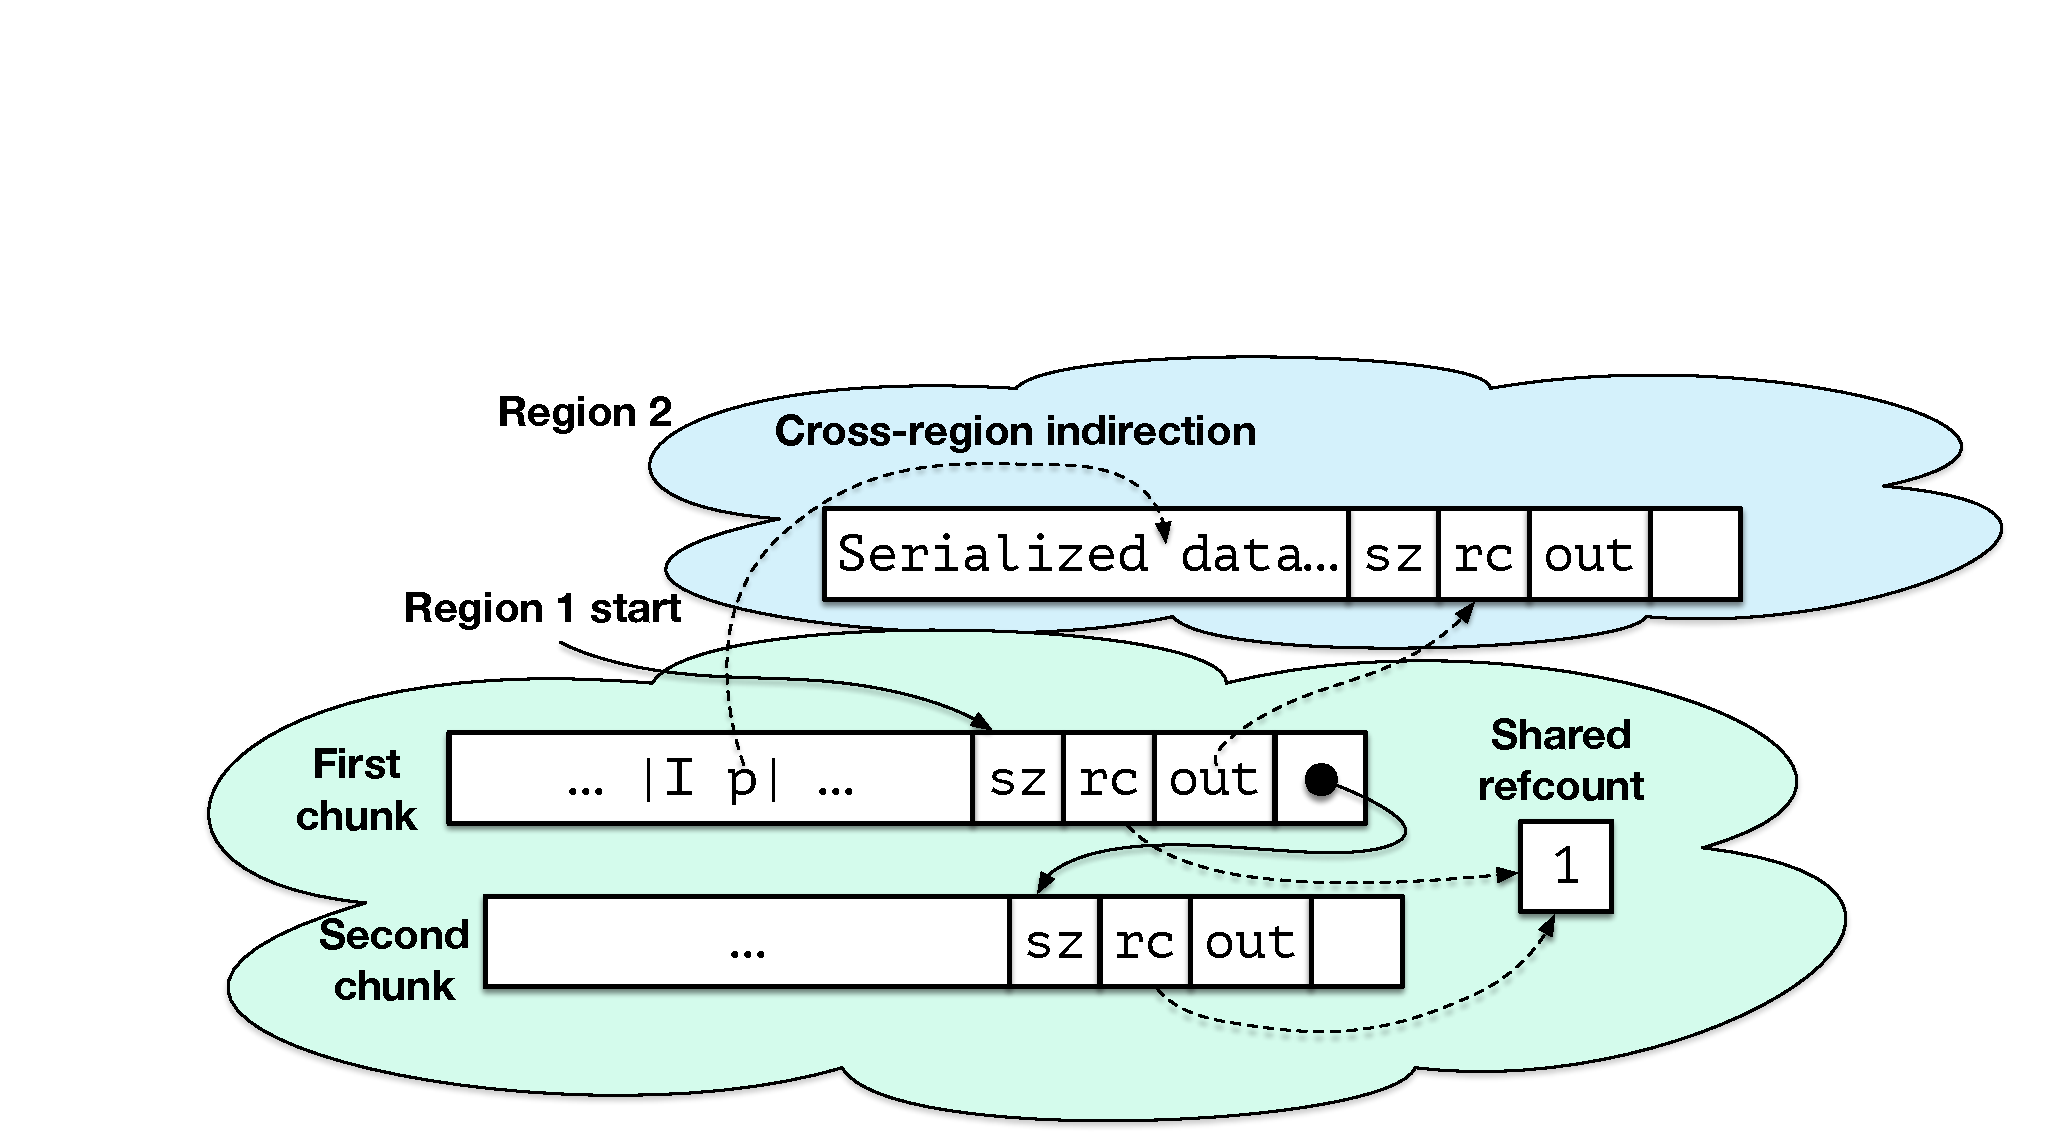
\includegraphics[width=0.75\textwidth]{region-memlayout2}
  \end{center}
  \vspace{-4mm}
  \caption{Example of multiple chunks making up a region, and of an inter-region
    indirection.  \captionscrunch{}}
  \label{fig:regions}
\end{figure}


\paragraph{Comparing against prior art's memory management}
Finally, in order to compare against other work, we also implement a technique
for {\bf huge regions}; these are allocated as a large slab containing many
pages, and could be extended by mapping new virtual memory after hitting a guard
page capping the region end.  This was the approach used by
Gibbon~\cite{ecoop17-gibbon}.
%
These huge regions avoid bounds checks when writing payloads and they are
suitable for programs with a small number of large regions (especially a single
input and single output region).  But they are inappropriate for the more
general case where programs may have small and short-lived regions.
%
%% \Red{We quantify the performance impacts of this trade-off in
%%   \secref{sec:eval-litmus}.}

%% Previous compilers based on regions, such as the MLKit compiler~\citep{mlkit},
%% can represent an extreme

The choice of allocation strategy can be informed by static information the
compiler gathers about the lifetime and potential size range of the region.  For
example, the region-based MLKit compiler achieved significant speedups from
statically classifying a majority of regions as constant-sized
\cite{mlkit-retrospective}, in which case they are allocated inside the procedure
stack frame.
%
% In our case, because we are packing many logical values into a smaller number of
In our approach, we unbox constant-sized data types (e.g. numbers), and
pack recursive data-types into growable regions, so we do not observe the same
opportunity for constant-sized regions.


%% \begin{itemize}
%% \item {\bf Bounds-check} or {\bf guard page}:
%% \item {\bf Copying} or {\bf Linking}:
%% \end{itemize}

%% The latter choice is relevant to the design of our ``mostly serialized''
%% representation, because {\em contiguity} changes the design space for
%% offset-based pointers.  For instance, if using the copying strategy


\section{Applications and Evaluation}
\label{section:applications}
\mav{General overview of the kinds of things we tested in Gibbon, how fast they were, etc.}

\subsection{Microbenchmarks}

See \tabref{tab:litmus-table}.

We are
% gibbon pointer cnf capn
202 / 2.6 / 3.2 / 9.4  $\times$ geomean faster than
Gibbon/NonPacked/CNF/CapNP respectively, and
0.96 / 2.6 / 3.2 / 7.3 $\times$ faster for only apples-to-apples asymptotics.
%% $3.2\times$,
%% $9.4\times$, and
%% $202\times$


%% \tabref{tab:litmus-table} shows the results.

\mav{Re-write to either remove or better explain difference between Gibbon1 and Gibbon2.}

The column labeled ``Gibbon2'' shows performance of \lamadt programs
(low-level \ourcalc control was not needed for any of these)
using indirections and offsets, automatically.
%
``Gibbon1'' shows the approach described in \cite{ecoop17-gibbon}.
%
There are two major sources of overhead for our new approach versus Gibbon1:

\begin{enumerate}
\item Growable regions:
In each case, our compiler starts with smaller, growable regions\footnote{starting at 64K bytes},
which we require to create small output regions as
in {\bf id} or {\bf treeInsert},
but we suffer the overhead of bounds-checking. On the other hand,
Gibbon always stores fully serialized data in huge regions.

\item Likewise, we have found that the backend C compiler is sensitive to the number
of cases in switch statements on data constructor tags (for instance, triggering
the jump table heuristic).  By including the possibility that each tag we read
may be a tagged indirection,
% or end-of-chunk,
we increase
code size and increase the number of cases in our switch statements.
\end{enumerate}


However, the benchmarks where indirections and random-access offsets are important (id,
rightmost, treeInsert, findMax) show a huge difference between Gibbon1 and Gibbon2,
as we would expect based on Gibbon1
requiring additional traversals to compile those functions.

\paragraph{Versus pointer-based representations}
The ``NonPacked'' approach is \ourcalc configured to always insert indirections
and thus emulate a traditional object representation.
% example of a traditional compilation approach
% that use one heap object per data constructor.
%
In this case, we are being overly friendly to this pointer-based representation by
allowing it to read its input (for example, the input tree to {\bf treeInsert})
in an already-deserialized, pointer-based form.  A full apples-to-apples
comparison would force the pointer-based version to deserialize the input
message and reserialize the output; but we omit that here to focus only on the
cost of the tree traversals themselves.
%
%% Similarly, the earlier Gibbon work compared a subset of these programs against a
%% larger set of traditional compilers (Java, gcc, GHC, OCaml, MLton, Racket, Chez),
%% finding those compilers performance on
%% pointer-based inputs worse than the performance of lifted functions on
%% serialized inputs.

\paragraph{Versus competing libraries}

%% The CNF representation is just the traditional Haskell heap representation of
%% data constructors.  It wastes a word of header space for garbage collection
%% purposes, and it uses full 64-bit absolute pointers between heap objects.
%% The result is fast to read but not space efficient.
%% This is visible on benchmarks such as {\bf sumTree}, where CNF out-performs
%% Cap'N Proto by $3.5\times$.
%% % (/ 0.96 0.27)
%% Conversely, the Cap'N Proto representation is space efficient---using 40\% fewer
%% bytes for the binary tree---and faster to build.
%% % (- 1 (/ 805 1340.0))
%% %
%% CNF results are slow to build because they involve an extra copy: first to
%% create the data on the normal heap, second to copy it into the compact region.
%% This is why CNF's {\bf copyTree} is twice as fast as {\bf add1Leaves}, even
%% though the both computations walk the tree and build a new output tree, copy is
%% able to use a runtime system function to walk the data and copy directly from
%% input message to output message, without allocating on the regular (non-compact)
%% Haskell heap.

The biggest differences in \tabref{tab:litmus-table} are due
asymptotic complexity.
However, for constant factor performance, we see the expected
relationship---that our approach and Gibbon are faster than CNF and Cap'N Proto,
sometimes by an order of magnitude, \eg\,{\bf add1Leaves}.

CNF and Cap'N Proto encode some metadata in their serialization, to
support the GHC runtime, and protocol evolution, respectively.
On the other hand,
our compiler only uses offsets and tagged indirections
when needed, and the size ratio of the encodings depends on how much these features are used.
%
For example, {\bf rightmost} uses a data-encoding that includes random-access
offsets, and {\bf treeInsert} creates an output with a logarithmic number of
tagged indirections.  Thus while our size advantage over CNF is
%
$4\times$ smaller
% (/ 1340.0 335)
%
on {\bf buildTree}, it is only
%
$2.22\times$
% (/ 1340.0 603)
% (/ 1340000000.0 (+ 334000000 (* (- (expt 2 25) 1) 8)))
%
for {\bf rightmost}.
% , and $XYZ\times$ for {\bf treeInsert}.

CNF results are slow to build because they involve an extra copy: first to
create the data on the normal heap, second to copy it into the compact region.
This is why CNF's {\bf copyTree} is twice as fast as {\bf add1Leaves}, even
though the both computations walk the tree and build a new output tree, copy is
able to use a runtime system function to walk the data and copy directly from
input message to output message, without allocating on the regular (non-compact)
Haskell heap.

\paragraph{Composing traversals}

For offset-insertion, we allow the whole-program compiler to select the data
representation based on what consuming functions are applied to it.
%% In a more general setting (say, modular compilation, or messages received over
%% the network from program in another language), we would need to adopt
%% random-access nodes uniformly, which would, e.g., give {\bf leftmost} the same
%% small amount of overhead in its input tree as {\bf rightmost}.
In the presence of multiple functions traversing a single data structure,
any function demanding random access changes the representation for all of them.
% the ``weakest link'' determines how many random-access nodes are needed.
% compiler uses a data representation required to optimize the slowest one.
{\bf repMax} is one such example:
%\begin{code}[mathescape=true]
\il{ repMax t = propagateConst (findMax t) t}.
%\end{code} \vspace{-5mm}
%  repMax = propagateConst . findMax -- almost correct!
% Consider the {\bf repMax} program in which
Here {\bf findMax} only requires a partial scan (random access), but propagating
that value requires a full traversal.  In this case, the compiler would add
offsets to the datatype to ensure that `findMax' remains
logarithmic.
%
However, this causes the subsequent traversal (propagateConst) to slow
down, as it now has to unnecessarily skip over some extra bytes.  Likewise, if
we do not include findMax in the whole program, the data remains fully
serialized, which is why {\bf propagateConst} and {\bf findMax} run separately
take less than 440ms, but run together take 480ms.  Yet the latter time is still
6$\times$ and 9$\times$ faster, respectively, than CNF and Cap'N Proto!



 \begin{table*}
  \begin{center}
    \small
      \begin{tabular}{ |c|c|c|c|c|c| }
        \hline
        Benchmark & Gibbon2 & Gibbon1 & NonPacked & CNF & CapnProto\hspace{-1mm} \\
        \hline
        % CNF: 100M iterations, calling NOINLINE id' function from NOINLINE rep.
        %      That gives 8.0ns (Allowing rep to inline, but not ID, makes it 2.15ns)
        % capnp: iter=20M median of 9 trials
        % Gibbon2: 100M iterations

        % Speedup:
        % CNF: (/ 2.1 2.1) = 1
        % CapnProto: (/ 129 2.1) = 61.42
        % Gibbon1: 152380952
        % Pointer: (/ 0.93 2.1) = 0.44
        {\bf id}:
        time, & 2.1ns &  0.32s  &  0.93ns &  2.1ns   & 129ns  \\
        complexity   & $O(1)$   &  $O(N)$ & $O(1)$    &  $O(1)$  & $O(1)$  \\
        %  output size (bytes)  &        &         &           &  8       &   8     \\
        \hline

        % CNF: 100M
        % capnp: iters = 20M median of 9

        % Speedup:
        % CNF: (/ 44 17.0) = 2.58
        % CapnProto: (/ 376 17.0) = 22.11
        % Gibbon1: (/ 18.0 17.0) = 1.05
        % Pointer: (/ 26 17.0) = 1.52
        {\bf leftmost}:
        time,        & 17ns         & 18ns        & 26ns        &    44ns      & 376ns            \\
        complexity   & $O(log(N))$  & $O(log(N))$ & $O(log(N))$ & $O(log(N))$  & $O(log(N))$ \\
        input size (bytes) & 335MB  & 335MB       & 335MB       &    1.34GB    & 805MB             \\
        \hline

        % CNF: 100M iterations
        % capnpL iter=20M, median of 9 trials
        % capnpL iter=20M, median of 9 trials
        % Speedup:
        % CNF: (/ 47 175.0) = 0.26
        % CapnProto: (/ 482 175.0) = 2.75
        % Gibbon1: 297142
        % Pointer: (/ 19 175.0) = 0.108
        {\bf rightmost}:
        time,        & 175ns        & 56ms    & 19ns        &    47ns      & 482ns \\
        complexity   & $O(log(N))$  & $O(N)$  & $O(log(N))$ & $O(log(N))$  & $O(log(N))$  \\
        input size (bytes) & 603MB & 335MB    & 335MB       &    1.34GB    & 805MB            \\
        \hline

        %capn: median of 9 trails iter=1
        % Speedup
        % CNF: (/ 4.5 0.27) = 16.66
        % CapnProto: (/ 1.8 0.27) = 6.66
        % Gibbon1: (/ 0.24 0.27) = 0.88
        % Pointer: (/ 2.7 0.27) = 10
        {\bf buildTree}:
        time,               & 0.27s     &  0.24s    & 2.7s &  4.5s  & 1.8s   \\
        complexity,         & $O(N)$    &  $O(N)$   &  $O(N)$ & $O(N)$  &  $O(N)$ \\
        output size (bytes) & 335MB     &  335MB    &  1.34GB &  1.34GB &  805MB       \\
        \hline

        % CNF: median of 9 trials:
        % capnp: median of 9 trails iter=1
        % Speedup:
        % CapnProto: (/ 3.8 0.25) = 15.2
        % CNF: (/ 2.7 0.25) = 10.8
        % Gibbon1: (/ 0.24 0.25) = 0.96
        % Pointer: (/ 3.1 0.25) = 12.4
        {\bf add1Leaves}:
        time,               & 0.25s     &  0.24s  & 3.1s     & 2.7s    &  3.8s  \\
        complexity,         & $O(N)$    &  $O(N)$ & $O(N)$   & $O(N)$  &  $O(N)$ \\
        \hline
        % CNF: median of 9 trials:
        % capn: median of 9 trails iter=1
        % Speedup:
        % CNF: (/ 0.27 0.095) = 2.84
        % CapnProto: (/ 0.96 0.095) = 10.10
        % Gibbon1: (/ 67.0 95) = 0.70
        % Pointer: 8.5
            {\bf sumTree}:
            time,               & 95ms     & 67ms     & 0.81s   &  0.27s  &  0.96s  \\
            complexity,         & $O(N)$   & $O(N)$   & $O(N)$  & $O(N)$  &  $O(N)$ \\
            \hline
            %capn: median of 9 trials iter =1
            % Speedup:
            % CNF: (/ 1.1 0.2) = 5.5
            % CapnProto: (/ 1.9 0.2) = 9.4
            % Gibbon1: (/ 0.24 0.2) = 1.2
            % pointer: (/ 3.5 0.2) = 17.5
                {\bf copyTree}:

                time,               & 0.2s      & 0.24s   & 3.5s   &  1.1s   &  1.9s       \\
                complexity,         & $O(N)$    & $O(N)$  & $O(N)$ & $O(N)$  &  $O(N)$ \\

                \hline
                \hline
                % CNF: median of 9 iters
                %capn: median of 9 trils iter=1
                % Gibbon numbers: median of 9 trials
                % Speedup:
                % CNF: (/ 4.27 0.5) = 8.54
                % CapnProto: (/ 2.1 0.5) = 4.2
                % Gibbon1: (/ 0.49 0.5) = 0.98
                % Pointer: (/ 2.96 0.5) = 5.92
                    {\bf buildSearchTree}:

                                    & 0.5s      & 0.49s     & 2.96s   &  4.27s   &  2.1s         \\
                    complexity,          & $O(N)$    & $O(N)$    & $O(N)$  & $O(N)$   &  $O(N)$ \\
                    output size (bytes)  & 603MB     & 603MB     & 1.61GB  &  1.61GB  &  805MB      \\

                    \hline

                    % CNF iters=1M
                    % This one is 2.5us with iters=1000
                    %            1.24us with iters=200K
                    %            1.04us with iters=1M
                    % NonPacked iters=1M
                    %
                    % capnp iters=20M median of 9
                    % Speedup:
                    % CNF: (/ 1 0.69) = 1.44
                    % CapnProto: (/ 1.3 0.69) = 1.88
                    % Gibbon: 144927
                    % Pointer: (/ 0.92 0.69) = 1.33
                    {\bf treeContains}:
                    time,                & 0.69$\mu$s   & 0.1s  & 0.92$\mu$s  &  1$\mu$s    & 1.3$\mu$s \\
                    complexity,          & $O(log(N))$ & $O(N)$ & $O(log(N))$ & $O(log(N))$ & $O(log(N))$ \\
                    \hline

                    % CNF iters=200K
                    % Capn median of 9 , iter=1
                    % Gibbon2 iters = 3500000
                    % Speedup:
                    % CNF: (/ 3.5 0.87) = 4.02
                    % CapnProto: (/ 150 0.87) = 172.4
                    % Gibbon: 436781
                    % Pointer: (/ 2.5 0.87) = 2.87
                    {\bf treeInsert}:

                    time,                & 0.87$\mu$s  & 0.38s  & 2.5$\mu$s   &  3.5$\mu$s   &  150$\mu$s  \\
                    complexity,          & $O(log(N))$ & $O(N)$ & $O(log(N))$ & $O(log(N))$  & $O(N)$  \\
                    avg bytes added      & 677 bytes        &  603MB  & 856 bytes   &  848 bytes  & 805MB  \\
                    \hline

                    %capnp: median of 9 trails iters=1M
                    {\bf InsertDestructive}:
                                         &  NA   & NA   & NA   & NA  &  1.37$\mu$s       \\
                    complexity,          &       &      &      &     & $O(log(N))$ \\

                    \hline

                    % Gibbon2:   100M iters
                    % Gibbon1:   20 iters
                    % Pointer:   100M iters
                    % CNF:       100M iters
                    % CapnProto: 1M iters
                    % Speedup:
                    % CNF: (/ 75 206.0) = 0.36
                    % CapnProto: (/ 597 206.0) = 2.89
                    % Gibbon: 427184
                    % Pointer: (/ 41 206.0) = 0.199
                    {\bf findMax}:
                    time,                & 206ns        & 88ms    & 41ns        & 75ns         & 597ns        \\
                    complexity           & $O(log(N))$  & $O(N)$  & $O(log(N))$ & $O(log(N))$  & $O(log(N))$  \\
                    \hline

                    % Speedup:
                    % CNF: (/ 4.2 0.43) = 9.76
                    % CapnProto: (/ 2.8 0.43) = 6.51
                    % Gibbon: (/ 0.42 0.43) = 0.97
                    % Pointer: (/ 3.3 0.43) = 7.67
                    {\bf propagateConst}:
                                         & 0.43s  &  0.42s  &  3.3s   & 4.2s   & 2.8s   \\
                    complexity,          & $O(N)$ &  $O(N)$ &  $O(N)$ & $O(N)$ & $O(N)$  \\
                    \hline

                    % Speedup:
                    % CNF: (/ 4.3 0.48) = 8.9
                    % CapnProto: (/ 2.9 0.48) = 6.04
                    % Gibbon: (/ 0.51 0.48) = 1.06
                    % Pointer: (/ 3.2 0.48) = 6.67
                    {\bf repMax}:
                    time,                & 0.48s  & 0.51s   & 3.2s    & 4.3s    & 2.9s   \\
                    complexity,          & $O(N)$ & $O(N)$  & $O(N)$  & $O(N)$  & $O(N)$  \\

                    \hline
      \end{tabular}
    \end{center}
  \vspace{-3mm}
    \caption{Tree-processing functions operating on serialized data.
      %% We are
      %% % gibbon pointer cnf capn
      %% 202 / 2.6 / 3.2 / 9.4  $\times$ geomean faster than
      %% Gibbon/NonPacked/CNF/CapNP, and
      %% 0.96 / 2.6 / 3.2 / 7.3 $\times$ faster for only apples-to-apples asymptotics.
      %% %% $3.2\times$,
      %% %% $9.4\times$, and
      %% %% $202\times$
      %% \captionscrunch{}
    }
    \label{tab:litmus-table}

\end{table*}


\subsection{Data Processing Benchmarks}

\mav{Overview of how this technique can be applied to data processing programs.}
\mav{If data to be processed is already serialized then this avoids marshaling cost.}
\mav{If data to be processed is in some other format then we can still be faster by
  transforming the data into a format that is more efficient to process (like the JSON
  to byte array transformation necessary for the Twitter benchmark). And in these cases
  it is often still faster than libraries that are meant to process the data in its
  original form.}


\subsubsection{Twitter JSON Benchmark}

For a real data set, we
use Twitter metadata consisting of user ID's and hashtags for all tweets posted
in 1 month, and count the occurrences of the hashtag ``cats'' in this dataset.
Here we seek to replicate and extend the CNF experiment reported by
\cite{cnf-icfp15}.

The dataset is stored on disk in JSON format, and we use RapidJSON
v1.1.0 ({\footnotesize\url{http://rapidjson.org/}}) as a performance baseline: a widely
recognized fast C++ JSON library.
%
In \figref{fig:twitter_slowdown_plot}, we vary the amount of data processed,
up to 1GB.  (For each data-point, taking the median of 9 trials
ensures the data is already in the Linux disk cache.)
%
For fairness, all versions read the data via a single \il{mmap} call, plus
demand paging.

There are two RapidJSON versions. The ``lexer'' version never constructs an
object representing a parsed tweet, rather, it is a state-machine
that is able to count ``cats'' while tokenizing, {\em without parsing}.  It is
optimized to be as fast as possible for this particular JSON schema, with no
error detection (a non-compliant input would give silent failures and wrong
answers).
%
The ``parser'' version represents a more traditional and idiomatic situation use
of the library: calling the \il{.Parse()} method to produce a DOM object, and
then accessing its fields.
%
We have structured this benchmark to maximally advantage this parsing approach:
the 9,111,741 tweets processed in the rightmost data points of \figref{fig:twitter_slowdown_plot} are stored as one JSON object each, on each line of the input file.
%
Thus the data only needs to be read into memory once, and in a single pass the RapidJSON benchmark reads, parses, discards, and repeats.
%
Conversely, if the tweets were instead stored as a single JSON array, filling
the entire input file, then RapidJSON would have to parse the entire file
(writing the DOM tree out to memory, overflowing last level cache), then read
that same tree back into memory in a second pass to count hashtags.
%
Nevertheless, in spite of this single-pass advantage, our compiler achieves
6$\times$ and 12$\times$ speedup over RapidJSON lexer/parser.
%
We process the 9.1M tweets in 0.39s.


\begin{figure}
  \centering
  \input{twitter_slowdown_plot}
  \caption{Twitter data processing benchmark results}
  \label{fig:twitter_slowdown_plot}
\end{figure}

\subsubsection{Point Correlation}

\mav{Summarize Laith's point correlation benchmark (from ECOOP
  paper), updating the language to match the new terminology from
  LoCal.}
Point correlation  is a well-known algorithm used in data mining~\cite{gray2000n}:
given a set of points in a k-dimensional space, point correlation computes the number of points in that space  that lie within a
distance $r$ from a given point $p$.

% Rather than comparing each point in the space to the query point, one efficient way of searching such spaces is to store them in kd-trees~\cite{bentley75}. KD-trees are space-partitioning trees where the root of the kd tree represents the entire space, and each node's children represents a partition of that node's space into two subspaces.

% A kd-tree is a binary space-partitioning tree that in its simplest form  splits the space at each internal node into two sub-spaces
% around a split axes in one of the space dimensions, the left subtree stores the points to the left of the split access
% and the right subtree sotres the points to the right of the split access, the split axes alternates between the dimensions of
% the space at each level of the tree, when the number of the points in the subtree is one, a leaf node that stores
% that point is constructed.


In a naive implementation of point correlation, each point in the space needs
to be checked against the query point.
A more efficient approach is to use kd-trees~\cite{bentley75} to store the
points. KD-trees are space-partitioning trees where the root of the kd tree represents the entire space, and each node's children represents a partition of that node's space into two subspaces.
KD-trees allow the search
process to skip some regions in the space. By storing at each internal node
the boundaries within which all descendent points lies, the search process can
skip a subtree is a given point is far enough from the boundaries. As a
result, querying a kd-tree to perform point-correlation is $O(log\; n)$ instead
of $O(n)$. Note that it is exactly the process of ``skipping'' subtrees that
gives kd-tree-based point correlation its efficiency, but also that prevents a
normal packed representation from sufficing to implement the algorithm: there
is no way to skip past a subtree without performing a dummy traversal,
obviating the asymptotic performance gains.

We implemented both a standard pointer-based version of 2-point correlation in
C, as well as a version that operates over a packed representation augmented
with indirection pointers. Each interior node stores a rope-style
indirection pointer that maintains the size of its child subtrees. If a
traversal is truncated at that node, the cursor is incremented by the value in
that indirection pointer, skipping the subtrees and resuming traversal on the
rest of the tree.

\figref{fig:point_corr_plot} shows the speedup of the packed version
with respect to the standard pointer-based implementation for
different tree sizes. For each tree size, we ran 10 query points
through the tree. For small trees, the queries were performed 10000
times to produce sufficient runtime for accurate measurements. Each
experiment was performed 10 times, and the mean is reported.

For every tree size, the packed representation uses 56\% less memory
than the pointer-based trees. This reduction in memory usage has two
sources: nodes do not need to store left-child pointers; and more
efficient packing of data in the packed representation. For small
trees, the runtime performance of the packed and pointer versions are
comparable. For large trees, the packed version is up to 35\% faster
than the pointer-based version.

The relatively smaller performance improvement for this
benchmark versus the Twitter benchmarks is unsurprising. First, taking an
indirection means that any spatial locality gains from the packed
representation are lost, resulting in similar behavior to the
pointer-based version. Second, there is relatively more work to be
done per node in this benchmark, so the time spent in traversal of the
tree is relatively less, reducing the opportunity for improvement.


\begin{figure}
  \centering
  \input{point_corr_plot}
  \caption{Speedup of serialized implementation of point correlation versus
    pointer-based implementation.}
  \label{fig:point_corr_plot}
\end{figure}

\subsection{Abstract Syntax Trees}\label{subsec:ast}

\mav{This is where my results for ASTs will eventually go.}
\mav{I can maybe put the Racket count nodes benchmark in here too, as a kind of
  AST traversal.}

\subsection{Parallel Programming Benchmarks}\label{subsec:parallelbench}

\mav{Copy over the benchmark results from the parallel gibbon paper.}
\mav{Paraphrase a brief summary of parallel gibbon again, reference the
  earlier section in it.}
